\documentclass{article}
\usepackage[utf8]{inputenc}
\usepackage{graphicx}
\usepackage{caption}


\title{\textbf{A Fast Matching Algorithm for Graph-Based Handwriting Recognition}}

\author{Emin Sadikhov \\  \href{emin.sadikhov@ozu.edu.tr} 
   \and Esad Simitcioglu \\  \href{esad.simitcioglu@ozu.edu.tr} }
\date{Spring 2021}

\begin{document}

\maketitle

\begin{abstract}
    "A Fast Matching Algorithm for Graph-Based Handwriting Recognition" by Andreas Fischer, Ching Y. Suen, Volkmar Frinken, Kaspar Riesen, and Horst Bunke offers efficient solution for handwriting recognition using graph-based algorithm derived from Hausdroff distance method. Due to lack of graph-based recognition methods, solving this problem with graph-based approach haven't been previously considered. The proposed solution runs in quadratic time, faster than previously used Hungarian algorithm which approximated distance between two handwriting graphs which in turn resulted in cubic time."
\end{abstract}

\section{Introduction}
 In early attempts in handwriting recognition best way to represent objects were graphs due to their ability to model different parts of an object as well as their binary relations. But in early attempts they only build applications for single character recognition as shown in Figure 1.
 
\begin{figure}[h]
    \centering
    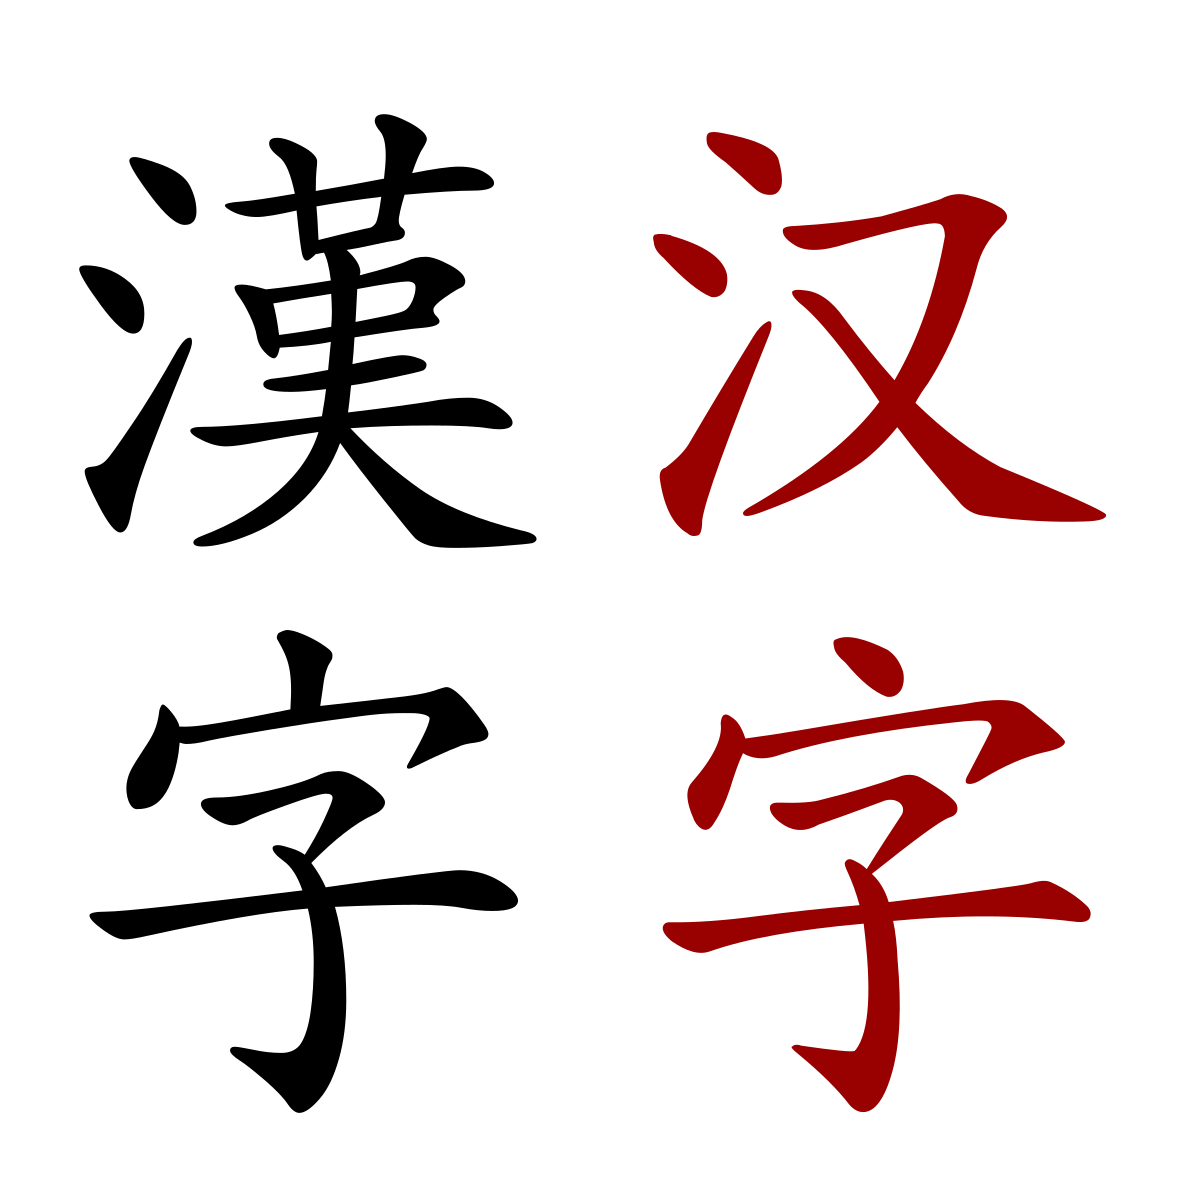
\includegraphics[width = .3\textwidth]{Images/Chinese.png}
    \caption{Chinese characters}
\end{figure}
 
 Today we specifically would like to detect unconstrained handwriting images that contain complete sentences. We can't use graphs in these sentences because of problems arising from the large variety of character shapes, the large number of words in natural language, and the inability to segment connected handwriting into characters before recognition. Existing systems are usually based on vectorial pattern representation and statistical classifier e.g. hidden Markov models and recurrent neural network. Recently, a general approach to bridging the gap between graph-based handwriting representation and statistical classification has been proposed [1]. With this approach the domain of the handwriting recognition change to graph-based approaches. We find the graph similarities between character prototype and handwritten character. Graph edit distance calculates the similarity. In the early days, Hungarian Algorithm was used to guess the approximate graph edit distance. However, time complexity of it was in cubic time with respect to the graph size. In this paper, Fischer et al. come up with a faster approach in calculating graph edit distance. Their solution reduced the time complexity to quadratic time with respect to the graph size. In this new and faster approach they used the Modified Hausdorff distance.
 

\section{Background}

Fischer et al. wants to find a new method to obtain graph edit distance. Previously it was done with Hungarian algorithm. Hungarian Algorithm was used to approximate the graph edit distance in cubic time with respect to the graph size. Even though the accuracy rate of the algorithm was very high, the algorithm was very slow; therefore, urging them to change the algorithm. They proposed a novel modification of the Hausdorff Distance called Modified Hausdorff Distance (HMM). In this section we will briefly explain some terms that are necessary to understand how HMM works.

\subsection{Graph Edit Distance}
Graph edit distance measures the minimum number of graph edit operations needed to transform one graph to another. Below are allowed graph edit operations:

\begin{description}
  \item[$\bullet$] Insert/Delete an isolated vertex
  \item[$\bullet$] Insert/Delete an edge
  \item[$\bullet$] Change the label of a vertex/edge\\
\end{description}


 \subsection{Hungarian Matching Algorithm}
 The Hungarian matching algorithm, also called the Kuhn-Munkres algorithm, is a $O$($|V|^3$) algorithm that can be used to find maximum-weight matchings in bipartite graphs, which is sometimes called as assignment problem. A bipartite graph can easily be represented by an adjacency matrix, where the weights of edges are the entries. 
 
 \subsection{Hausdorff Distance}
 In mathematics, the Hausdorff distance, measures how far two subsets of a metric space are from each other. It turns the set of non-empty compact subsets of a metric space into a metric space in its own right. Informally, two sets are close in the Hausdorff distance if every point of either set is close to some point of the other set. In other words, it is the greatest of all the distances from a point in one set to the closest point in the other set. Hausdorff Distance is widely used in the domain of image matching [3].



\begin{equation}
H(A, B)=\max \left(\max _{A} \min _{B} d(a, b), \max _{B} \min _{A} d(a, b)\right)
\end{equation}


Fischer et al. defines Hausdorff Distance as "only the maximum over all nearest neighbour distance is taken into account". Consider A as the nodes of the graph $g_1$ and B as the nodes of the graph $g_2$. So it calculates in $O(AB)$ where A and B denote number of the nodes in $g_1$ and $g_2$ respectively.

\begin{equation}
H^{\prime}(A, B)=\sum_{A} \min _{B} d(a, b)+\sum_{B} \min _{A} d(a, b)
\end{equation}

Equation 2, we called it faster alternative for approximate graph edit distance. It handles the exceptions like ink bleed. Equation 1, the Hausdorff Distance, is not paying attention to these exception. Hence, it is modified for handwriting recognition. Modified Hausdorff Distance gives us the far better performance than classic Hausdorff Distance method. We will further discuss these results in Section 4 (Figure 5).

 
\subsection{Approximate Graph Edit Distance}

Approximate Graph Edit distance is used to find the graph similarity between handwritten and prototype letter. This distance also includes minimum cost to convert handwritten $g_2$ to prototype $g_1$. In total, there are three possible operations for conversion which are substitution, insertion and deletion. Approximate graph edit distance is calculated by following formulas:


\begin{center}
$-c\left(n_{1}, n_{2}\right)=\left\|\left(x_{1}, y_{1}\right)-\left(x_{2}, y_{2}\right)\right\|$ for node label substitution\\ 

$-c\left(n_{1}, \epsilon\right)=c\left(\epsilon, n_{2}\right)=C_{n} \geq 0 $ for node deletion and insertion\\ 

$-c\left(e_{1}, \epsilon\right)=c\left(\epsilon, e_{2}\right)=C_{e} \geq 0 $  for edge deletion and insertion\\
\end{center}


For calculation of dissimilarity, the graph edit distance (Section 2.1) is required. Generally edit distance problems are calculated using $A*$ algorithms. One of the main reasons for its use, is its optimally and correctness. However, this decreases the efficiency of the algorithm; as a result,  $A*$ runs in exponential time which causes efficiency problems once the handwriting graphs gets bigger. To solve this inefficiency, Hungarian algorithm is used. 
Hungarian algorithm, as described in Section 2.2, uses approximation for solving edit distance. It converts the problem into simple node assignment problem similar to bipartite graph. Hungarian algorithm is faster than $A*$ and runs in cubic time, however, the downside of it, is that once the graph gets large, the accuracy of algorithm decreases due to approximation. Another drawback of the algorithm is that once the graph is converted to node assignment problem, the computation cost at the edge nodes are ignored. Again, they are approximated and the result of edit distance is \\ returned. 




\section{Main Section}
In this section we will try to explain the proposed algorithm. In section 3.1, we will give mathematical definitions and explanations followed by a visual example in section 3.2.


\subsection{Definitions}
Fischer et al. derives a faster graph matching method from the Hausdorff distance (Section 2.3). This Hausdorff distance method is different from the first Hausdorff Distance method (equation 1). The proposed Modified Hausdorff Distance preserves most properties of the approximate graph edit distance. It is based on node assignment according to some edit cost. By allowing multiple node assignments for the proposed method, the time complexity is reduced from cubic to quadratic with respect to graph size. In this section we will try to explain the proposed algorithm. \\

Novel modification of the Hausdorff distance (Section 2.3) with deletion and insertion cost is defined as 


\begin{equation}
H^{\prime \prime}(A, B)=\sum_{A} \min _{B} \overline{c_{1}}(a, b)+\sum_{B} \min _{A} \overline{c_{2}}(a, b)
\end{equation}

by replacing the metric $d$ in Equation 2 in Section 2.3 with cost functions $\overline{c_{1}}$ and $\overline{c_{2}}$. A corresponds with the nodes of graph $n_1$ and B with the nodes of $n_2$. The cost functions $\overline{c_{1}}(n_1,n_2)$ and $\overline{c_{2}}(n_1,n_2)$ for matching node $n_1$ with node $n_2$ are 

\begin{equation}
\bar{c}_{1}\left(n_{1}, n_{2}\right)=\left\{\begin{array}{ll}\frac{c\left(n_{1}, n_{2}\right)}{2}, & \text {if \;}  c\left(n_{1}, n_{2}\right)<c\left(n_{1}, \epsilon\right) \\ c\left(n_{1}, \epsilon\right), & \text { otherwise }\end{array}\right. 
\end{equation}

\begin{equation}
\overline{c_{2}}\left(n_{1}, n_{2}\right)=\left\{\begin{array}{ll}\frac{c\left(n_{1}, n_{2}\right)}{2}, & \text { if } c\left(n_{1}, n_{2}\right)<c\left(\epsilon, n_{2}\right) \\ c\left(\epsilon, n_{2}\right), & \text { otherwise }\end{array}\right.
\end{equation}

with respect to the cost function c of the edit distance (Section 2.4). That is $ \min _{B} \overline{c_{1}}(a, b)$ returns half of the node substitution cost $\frac{c(n_1,n_2)}{2}$ if the substitution $(n_1,n_2)$ is preferred over deletion $(n_1,\epsilon)$ of $n_1$. Among all possible substitutions the one with the smallest cost is chosen. Otherwise the deletion cost $(n_1,\epsilon)$ is returned. Similarly,  $ \min _{A} \overline{c_{2}}(a, b)$ returns the  best $\frac{c(n_1,n_2)}{2}$ if the substitution  $(n_1,n_2)$ is preferred over insertion $(\epsilon,n_2)$ of $n_2$. \\

If a substitution is preferred in $\overline{c_{1}}$ or to the $\epsilon$ node for deletion. Vice versa, each node of graph $g_2$ is either assigned to a node of graph $g_1$ if a substitution is preferred in $\overline{c_{2}}$ or to the $\epsilon$ node for insertion.

\subsection{Sample Scenario}





\begin{center}
\end{center}
\begin{figure}[h]
    \centering
    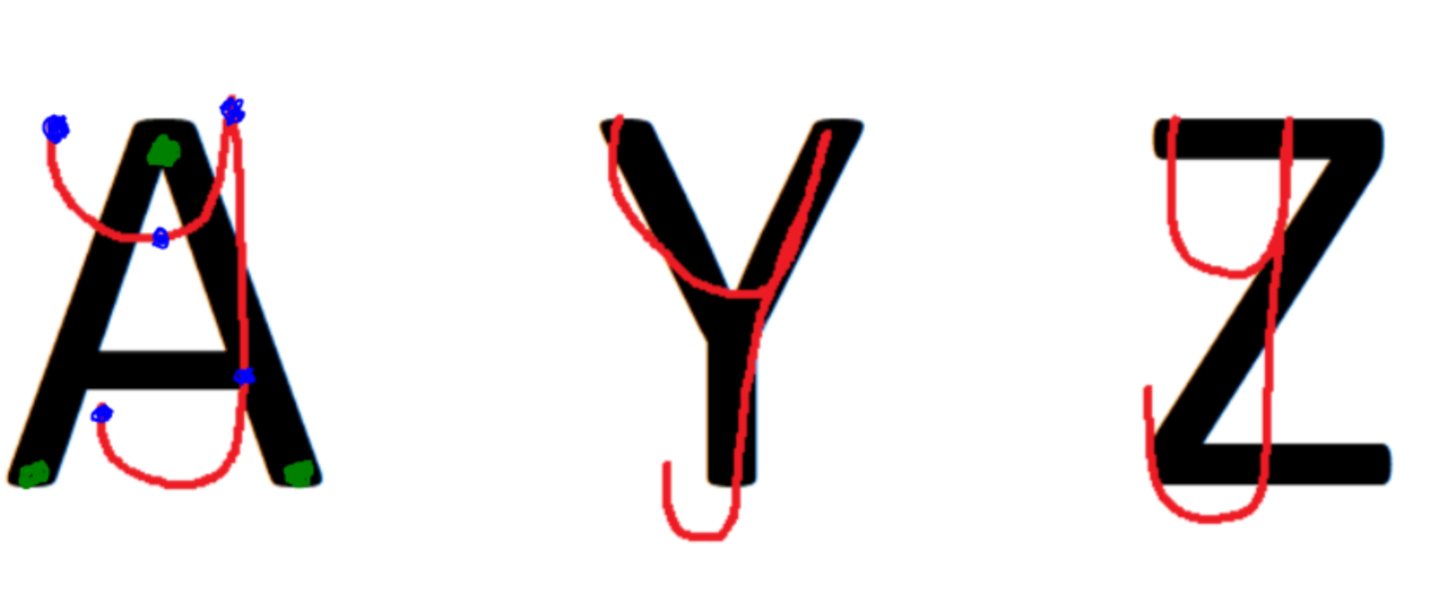
\includegraphics[width = .5\textwidth]{Images/over.png}
    \caption{Prototype Selection}
\end{figure}

Algorithm puts the handwritten letter on the prototype as shown in Figure 2. Also,both handwritten and prototype letters are in graph representation. You can think that both prototype and handwritten letters are converted to a graph and every corner edge (nodes in blue color in Figure 2) of the graph has a node. Next, the algorithm compares the distances between the nodes of the handwritten letter and the nodes of the proposed prototype. Algorithm does this process for all possible prototypes letters in alphabet (A - Z) and picks the one with the least distance as a solution. 

\begin{center}
\end{center}
\begin{figure}[h]
    \centering
    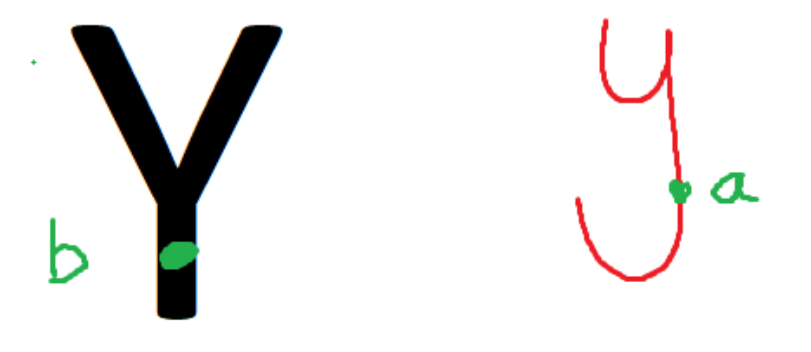
\includegraphics[width = .5\textwidth]{Images/node_comparision.png}
    \caption{Transform of Graph}
\end{figure}

After successfully finding the prototype, the algorithm will need to transform handwriting to that prototype. Algorithm will pick the operation with the least cost. In Figure 3 you can see the node comparison. Selected operation might be substitution of node $a$ to node $b$ (with insertion or deletion operations). If we can change the node $a$ with a small cost of insertion or deletion operation, the algorithm will chose this option. Otherwise, it might be just a copy operation of node $b$ to node $a$. If we can't transform the node $a$ to node $b$ node easily, we need to copy the node $b$ to exact position of the node $a$ which will be more costly operation.

% \clearpage

\begin{center}
\end{center}
\begin{figure}[h]
    \centering
    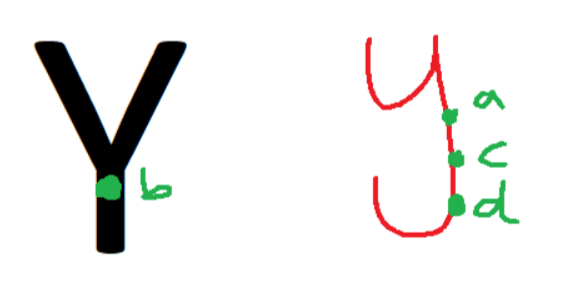
\includegraphics[width = .5\textwidth]{Images/yeni.png}
    \caption{Advantage of Modified Hausdorff Distance}
\end{figure}

Modified Hausdorff Distance algorithm only uses the graph edit distance for computation of minimum cost, once there is a change in the node order. If the nodes are along a straight line the cost calculation will be same for all of them. Therefore, Modified Hausdorff Distance computes the minimum cost once it detects a corner edge or a change in the order of the nodes. This significantly improves the efficiency of algorithm since unnecessary computations are ignored. However, as you can guess the accuracy rate will be lower compared to Hungarian algorithm, but the decrease won't be significant statistically.

\section{Discussion}

\begin{center}
\end{center}
\begin{figure}[h]
    \centering
    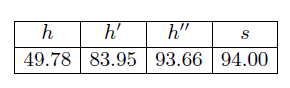
\includegraphics[width = .4\textwidth]{Images/test.png}
    \caption{Word recognition accuracy on the test set in percentage}
\end{figure}

As you can see from Figure 5 Hausdorff Distance (which represented as h) gives a low accuracy. That's why they can't use this algorithm as raw. In time, Hausdorff Distance had an improvement (which is represented as h'). It increased the rate nearly  twice as h but still it didn't satisfy the Fischer et al. The best accuracy rate was achieved with graph similarity features and approximate edit distance methods which is represented as s in figure 5. It kills the traditional statistical feature sets which achieve maximum accuracy of 90.48\% [1]. The proposed algorithm increases the efficiency by almost keeping the recognition accuracy the same as it was with Hungarian algorithm. The accuracy rate is negligibly lower because The Modified Hausdorff Distance method doesn't calculate the dissimilarity for all the nodes. If the letter has no edge or corner then there is no need to calculate that node again (You can see an example in Figure 4). With this improvement it gains speed but loses accuracy rate. There is no statistically significant difference between the results. 

\begin{center}
\end{center}
\begin{figure}[h]
    \centering
    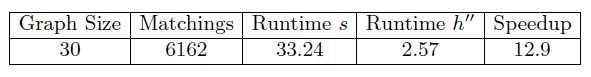
\includegraphics[width = .8\textwidth]{Images/result.png}
    \caption{Runtime statistics}
\end{figure} 

You can see the improvement of the proposed algorithm in Figure 6. You can see the run-time difference between s and h''. It is amazing to get this result without losing significant accuracy rate. The proposed algorithm achieves a speedup factor of 12.9. Now we can understand the true power of the Modified Hausdorff Distance.


\section{Conclusion}
In Handwriting, recognition graphs was not the first choice to represent. Then the gap between graph-based handwriting representation and statistical classification has been proposed in [1]. So Graph Similarity features started to be used in this topic. Hungarian Algorithm shows us a big accuracy rate for handwritten inputs, however, the cubic run-time for approximation of graph edit distances (Section 2.1) significantly decreases the efficiency of the algorithm [2]. In this paper, Fisher et al. proposes a fast matching algorithm named Modified Hausdorff Distance, derived from the Hausdorff Distance. They reduce the time complexity from cubic time to quadratic time without significant loss in the accuracy rate. In Figure 6 you can see that speedup factor of the new proposed algorithm is 12.9.

For future work, we need to verify that this efficiency is preserved with other graph data sets. Maybe with more complex graphs, this speedup factor can be changed. In short, this algorithm needs to be tested for other scenarios. Then, there can be a method which solves the proposed distance much better and we can find a different and even more efficient variant of Hausdorff Distance. The power of Hausdorff Distance doesn't have to be tied to just one subject. If someone can finds that method it will be game changing for domain of handwriting recognition.  

\clearpage

\begin{thebibliography}{9}

\bibitem{fromTheArticle} 
Fischer, A., Riesen, K., Bunke, H.
\textit{Graph similarity features for HMM-based
handwriting recognition in historical documents. In: Proc. 12th Int. Conf. on
Frontiers in Handwriting Recognition}. 2010

\bibitem{fromTheArticle} 
Munkres, J.
\textit{Algorithms for the assignment and transportation problems. Journal
of the Society for Industrial and Applied Mathematics}. 1957

\bibitem{fromTheArticle} 
Huttenlocher, D.P., Klanderman, G.A., Kl, G.A., Rucklidge, W.J.
\textit{Comparing
images using the Hausdorff distance. IEEE Trans}. 1993

\bibitem{geeksforgeeks} 
Rachit Belwariar.
\textit{A* Search Algorithm}. 2021
\\\texttt{https://www.geeksforgeeks.org/a-search-algorithm/}

\bibitem{hungarianmethod} 
Karleigh Moore, Nathan Landman, and Jimin Khim. 
\textit{Hungarian Maximum Matching Algorithm}
\\\texttt{https://brilliant.org/wiki/}

\bibitem{hungarianmethod} 
Kaspar Riesen , Horst Bunke 
\textit{Approximate graph edit distance computation by means of bipartite graph matching}. 2008


\end{thebibliography}


\end{document}